% kapitel2.tex
%\chapter{Die Softwarekonstruktion}
%\label{chapter:kap2}
\section{Aufbau der Softwarearchitektur}
Wie im ersten Teil der Ausarbeitung verdeutlicht wurde, ist der Raspberry Pi im Inneren des Spiegels das Kernstück der gesamten Plattform. Auf dieser Hardwarekomponente läuft dementsprechend die komplett entwickelte Software. 

Das Softwareprojekt selbst ist in zwei Komponenten aufgeteilt. Die erste Softwarekomponente realisiert die eigentliche SmartMirror-Anwendung inklusive der Ausgestaltung der Benutzungsschnittstelle, der Kommunikation mit verbauten Sensoren und des Datenimportes aus Datenquellen des Internets. Diese Anwendung ist in Python geschrieben, realisiert die SmartMirror-Funktionalität und hat den größten Anteil des Implementierungsaufwandes erfordert. Im Gegensatz dazu steht die zweite Softwarekomponente, im folgenden StartUp-Anwendung genannt, die ein Skript umfasst, das nach dem Systemstart die SmartMirror-Anwendung startet. Bei dieser handelt es sich eher um eine erforderliche Hilfskomponente von geringerem Umfang, die als Bash-Skript direkt ausführbar auf Betriebssystemebene realisiert wurde.  

\begin{figure}
	\centering
	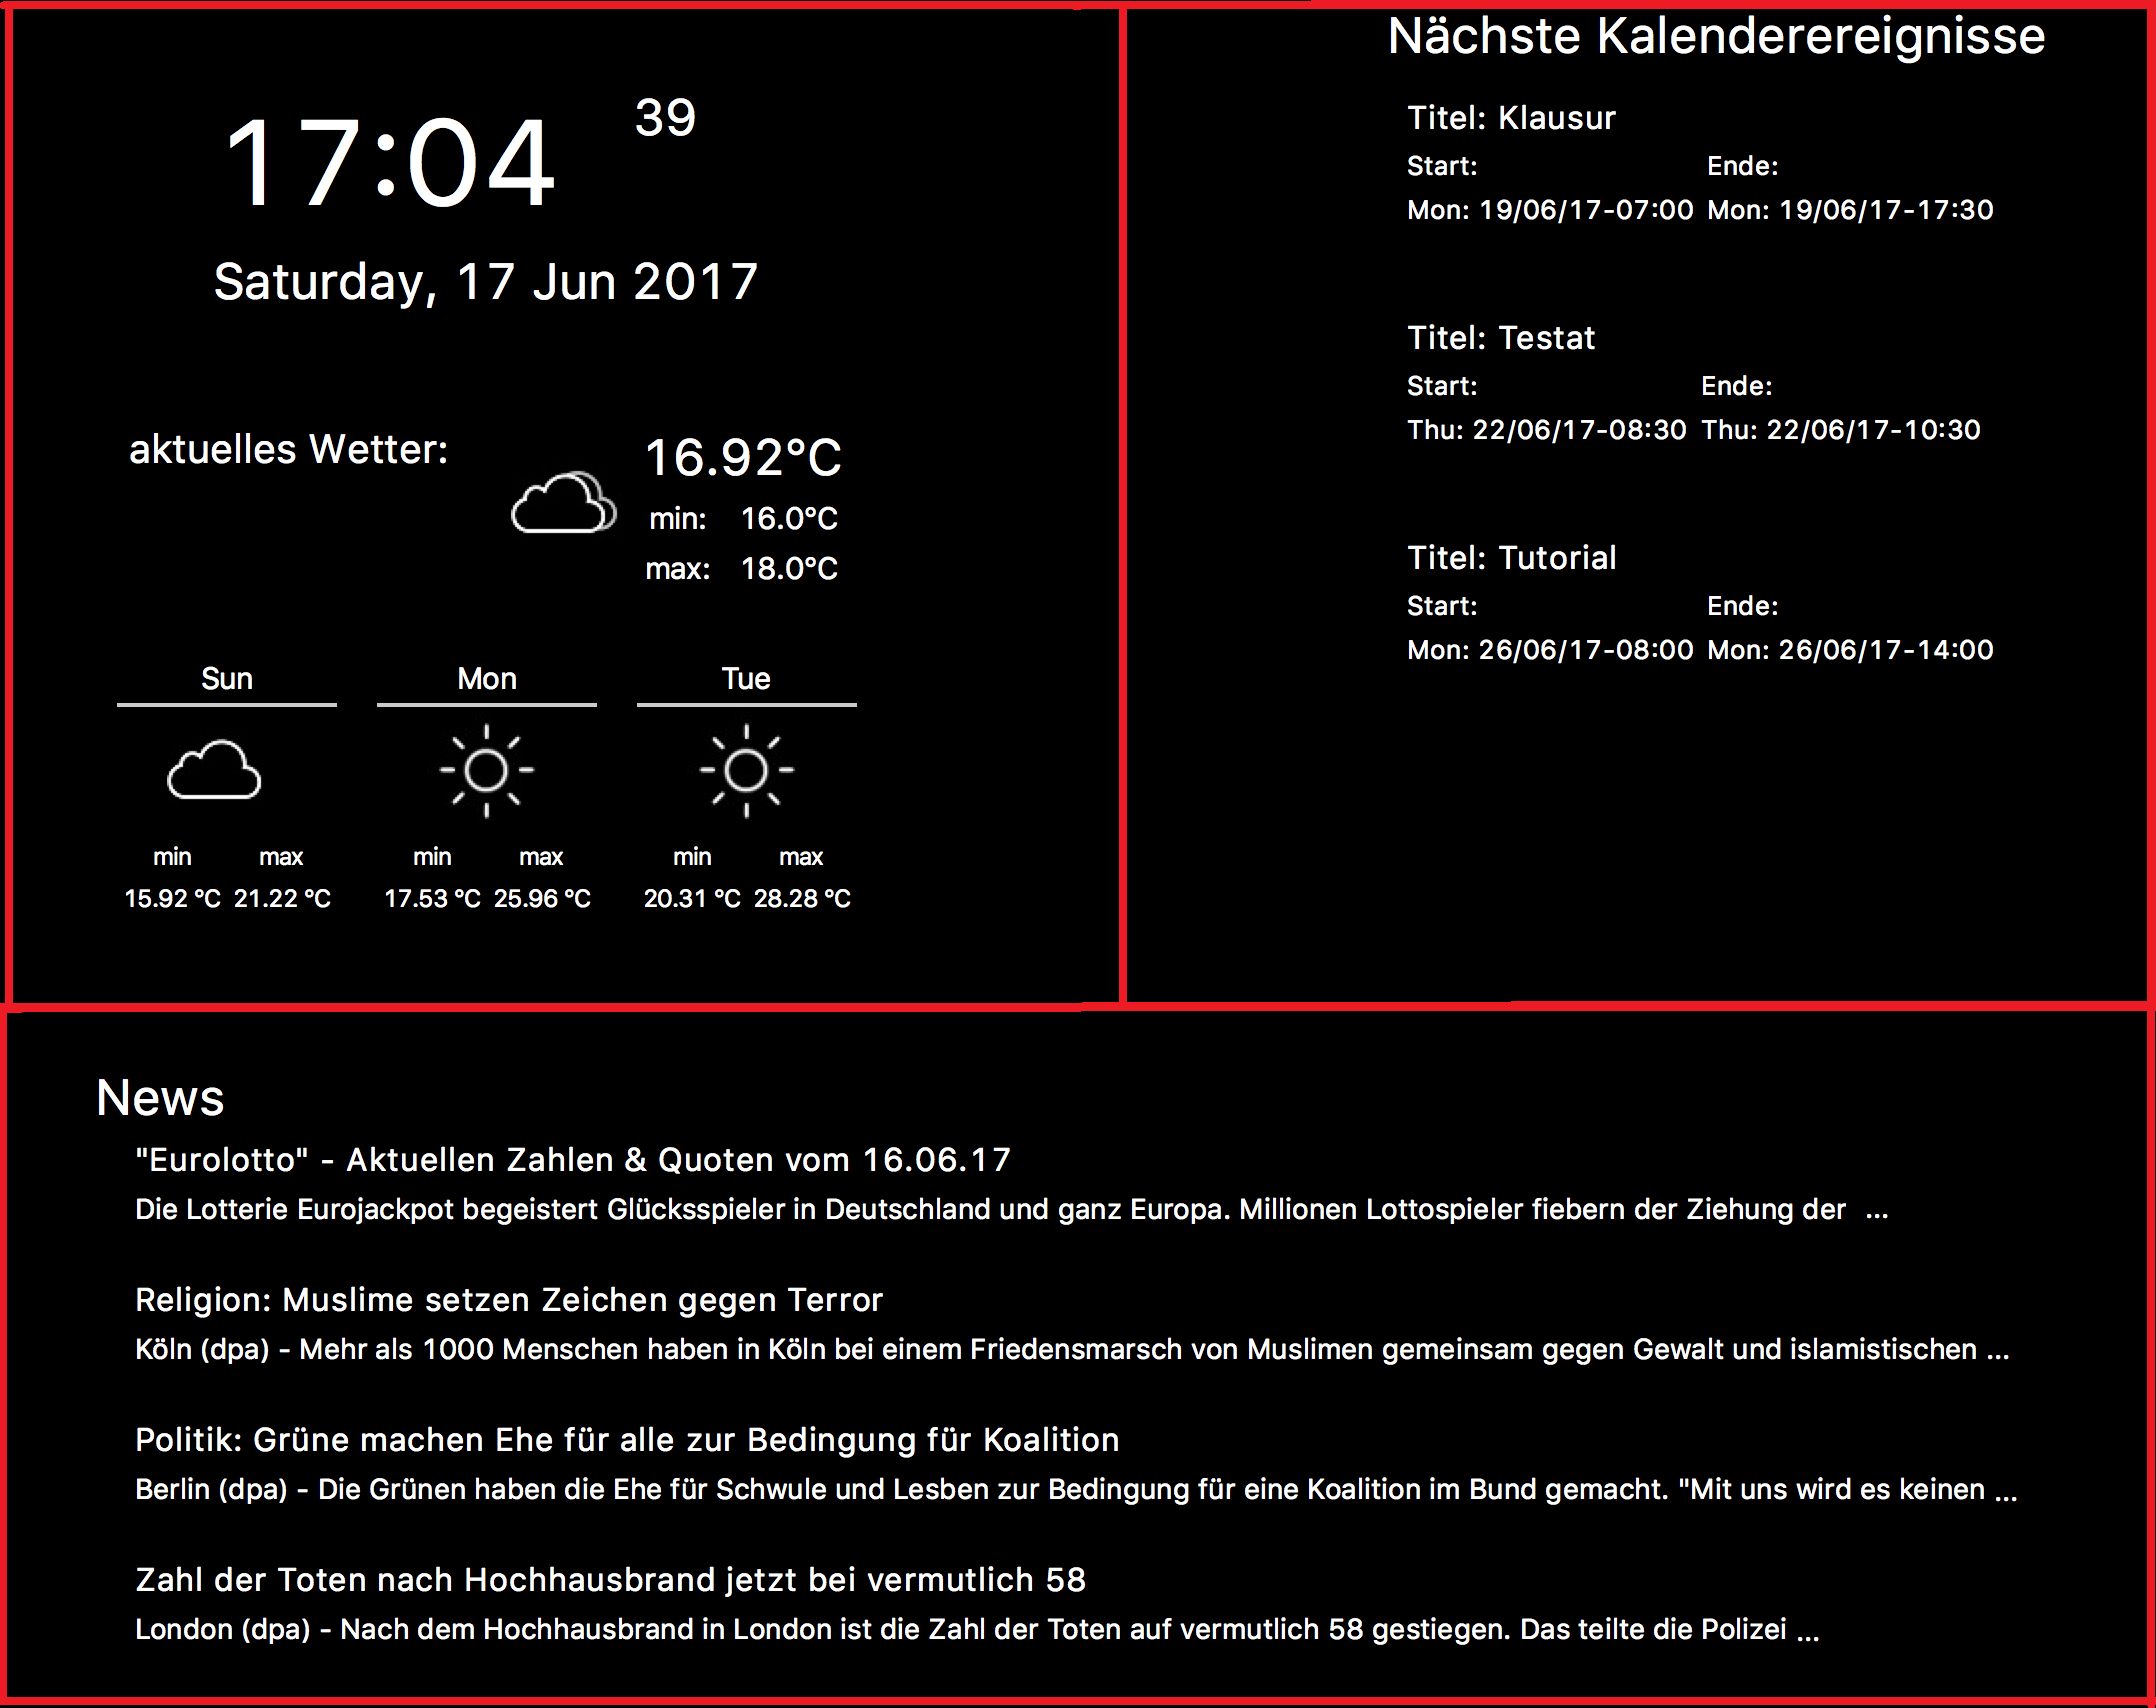
\includegraphics[width=0.7\linewidth]{bilder/grafOberflaeche}
	\caption[Verteilungsdiagramm der SmartMirror-Applikationen]{Verteilungsdiagramm der SmartMirror-Applikationen}
	\label{fig:verteilungsdiagramm}
\end{figure}

Zum besseren Verständnis ist in \autoref{fig:verteilungsdiagramm} der softwaretechnische Technologiestack der beiden Softwarekomponenten in Form eines UML-Verteilungsdiagramms dargestellt (Literatur). Die zentrale physikalische Ausführungseinheit ist der Raspberry Pi. Dieser kommuniziert über das Serial IO-Protokoll (SIO) mit den zwei verbauten Sensoren: einem Bewegungssensor, sowie einem kombinierten Temperatur- und Luftfeuchtigkeitssensor. Beide Sensoren wurden so gewählt, dass eine Kommunikation über SIO möglich ist. Dieses Protokoll lässt sich über die ...-API (Literatur) sehr gut in Phython-Anwendungen einbinden, wie im \autoref{subsec:kommunikation} weiter ausgeführt wird. Des weiteren zeigt das Diagramm, dass zwei weitere Informationsquellen über das Internet, also das http(s)-Protokoll, angebunden werden. Dabei handelt es sich zum Einen um  
einen Newsserver (XYZ-Adresse?!), über den aktuelle Spiegel-Nachrichten über einen RSS-Feed (Literatur) eingebunden werden können und zum Anderen um die Einbindung eines google-Kalenders. Die Kalendereinträge werden über  REST-Webservices (Literatur) im JSON-Format (Literatur/Quelle) abgefragt. 

Die beiden Softwarekomponenten des SmartMirrors laufen auf Basis eines Linux ..., das als Betriebssystem auf dem Rasberry Pi installiert wurde. Die SmartMirror-Anwendung \glqq SmartMirror.??? \grqq ist ein Artefakt, welches durch den Python-Interpreter \glqq XYZ \grqq interpretiert wird. Das StartUp-Skript kann mit dem Kommando \glqq .... \grqq direkt auf dem Betriebssystem ausgeführt werden. 

Beide Softwarekomponenten werden im Folgenden detaillierter beschrieben: zuerst die SmartMirror-Anwendung und dann das StartUp-Skript.

\begin{figure}
	\centering
	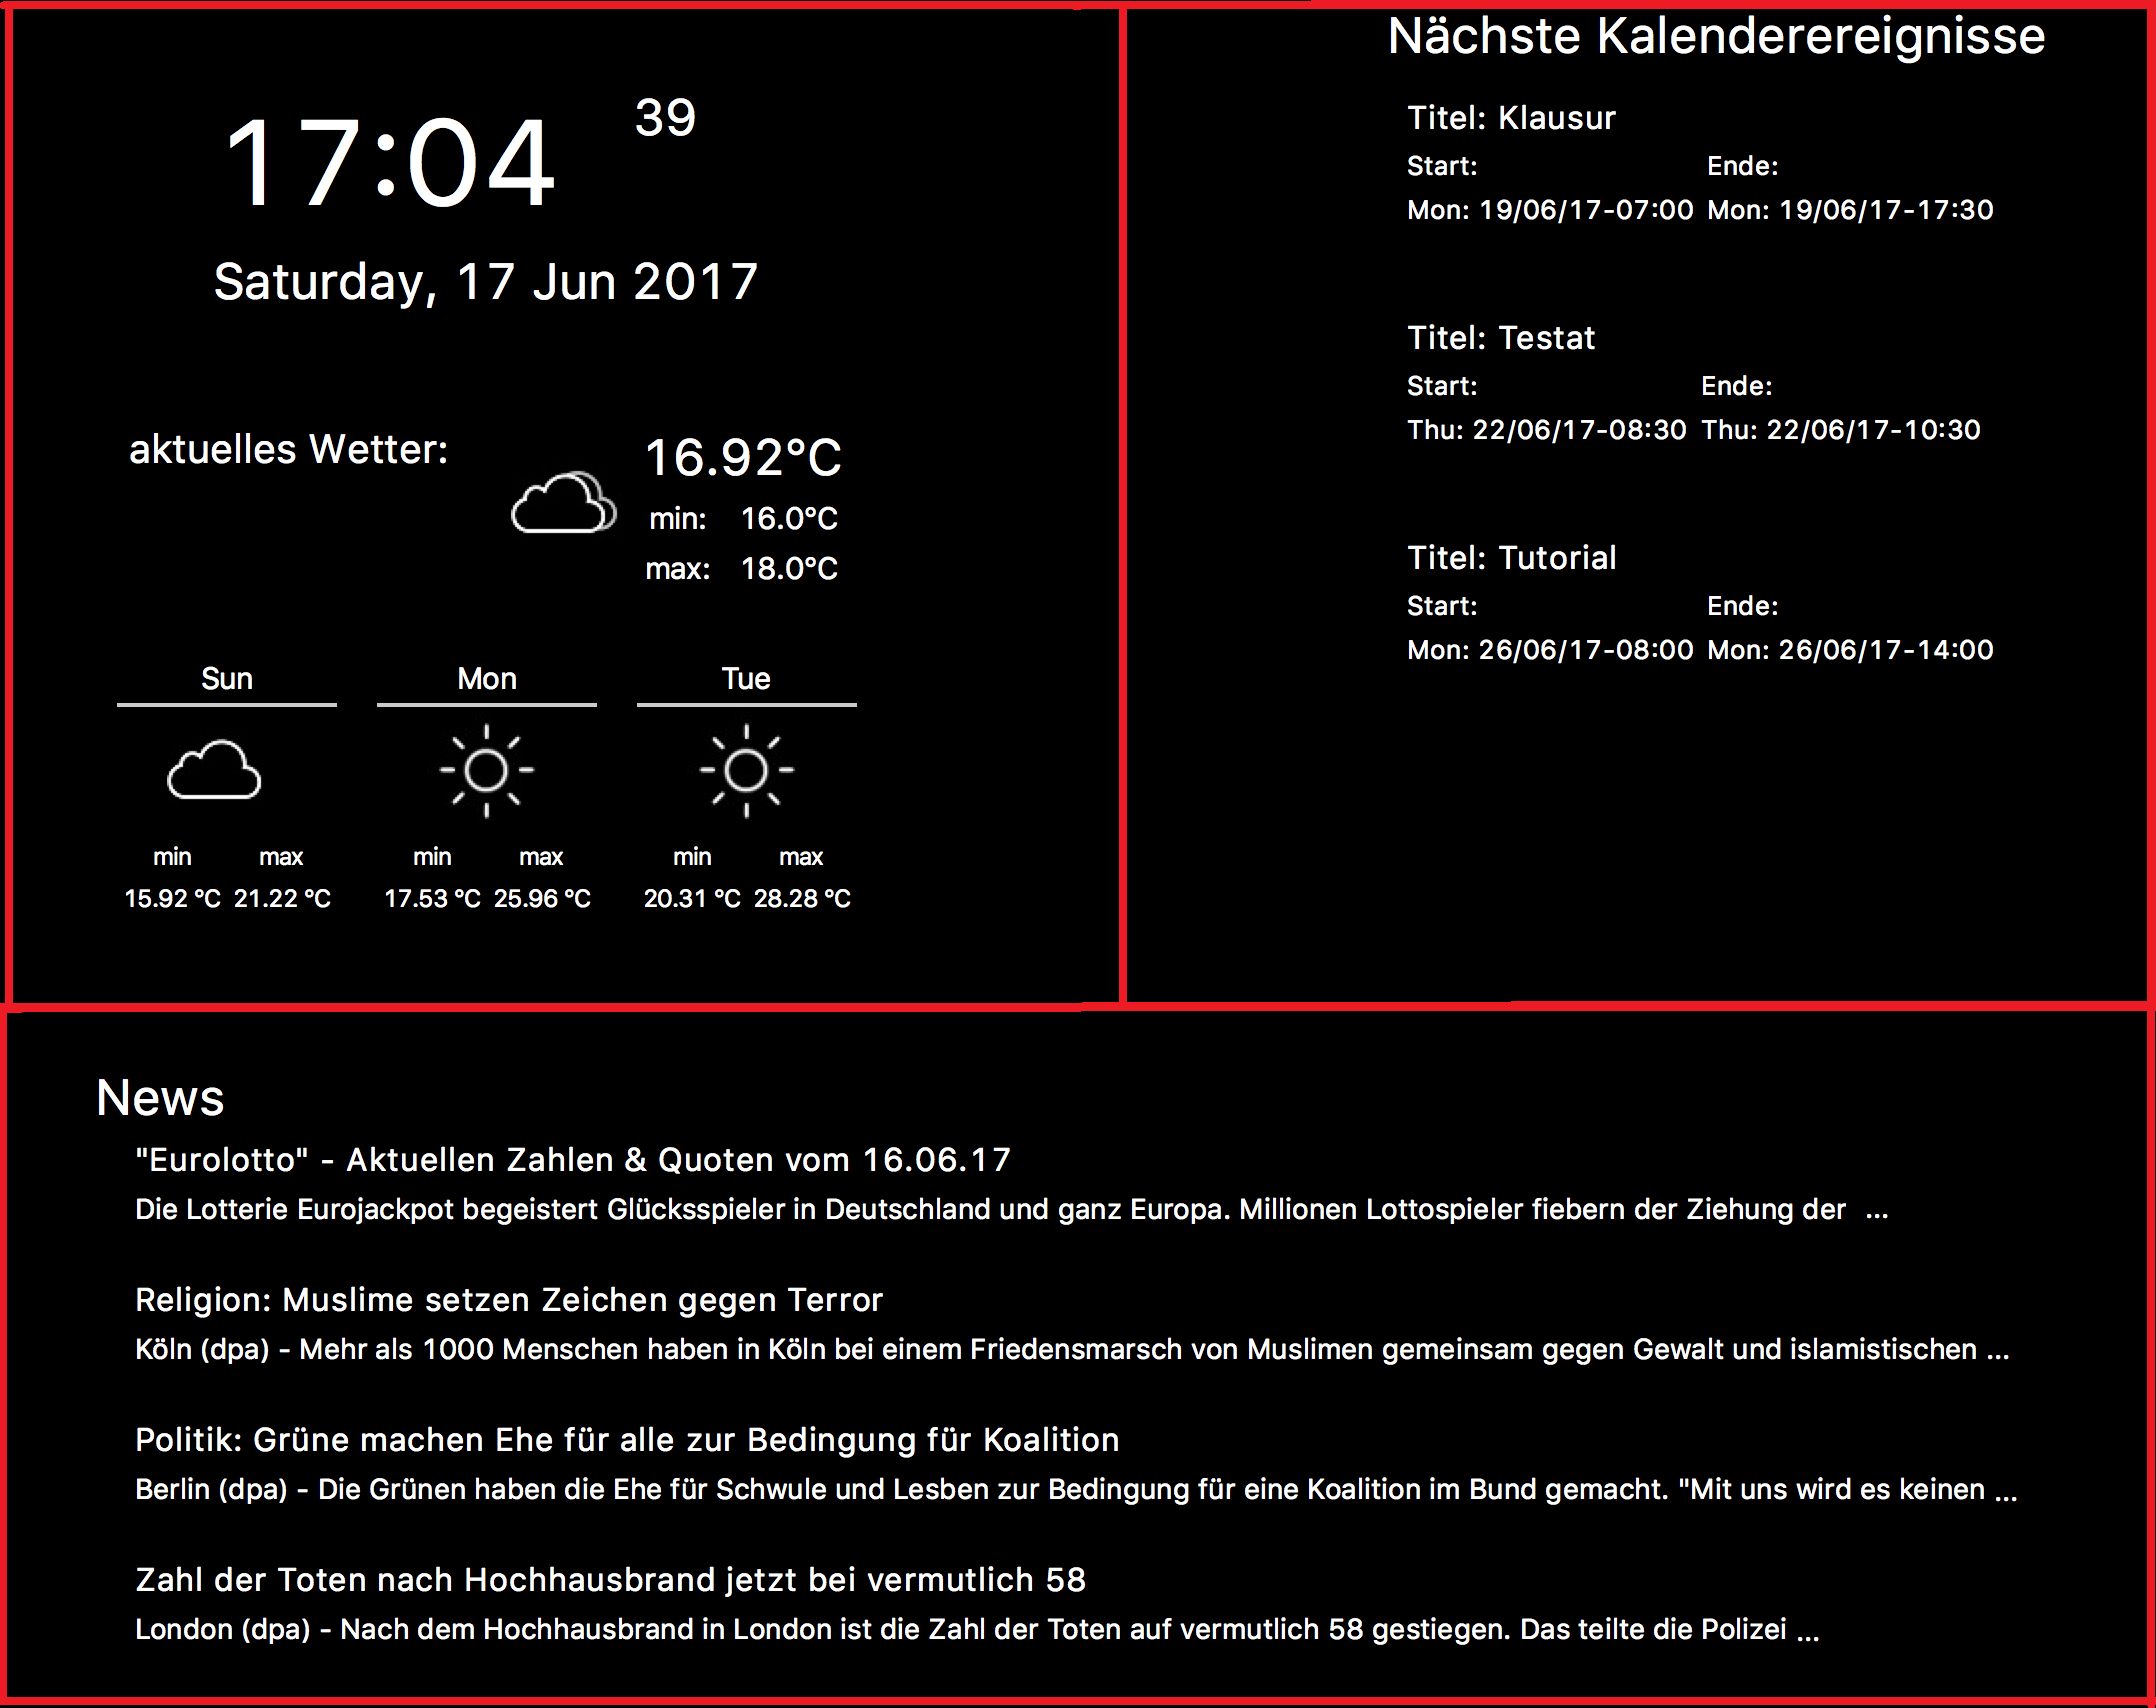
\includegraphics[width=0.7\linewidth]{bilder/grafOberflaeche}
	\caption[Benutzungsschnittstelle der SmartMirror-Anwendung]{Benutzungsschnittstelle der SmartMirror-Anwendung}
	\label{fig:grafoberflaeche}
\end{figure}


\subsection{Die SmartMirror-Anwendung}

Die Funktionalität der SmartMirror-Anwendung lässt sich am besten ausgehend von der Gestaltung der Benutzungsschnittstelle erfassen, die in \autoref{fig:grafoberflaeche} dargestellt wird. Die Darstellung lässt sich grob in drei Bereiche strukturieren: den oberen linken Bereich, den oberen rechten und den unteren Bereich. Oben links werden aktuelle Informationen konkret Uhrzeit, Datum und Wetterdaten angezeigt, während im rechten Bereich die nächsten Kalenderereignisse (bzw. ToDos) aufgeführt werden und im unteren Bereich aktuelle Neuigkeiten (News) angezeigt werden. 

\subsubsection*{Benutzungsschnittstelle}

Zur Gestaltung der Benutzungsschnittstelle wurde das Framework TkInter genutzt. Die Abkürzung steht für (\textbf{Tk Inter}face).  Durch Tkinter ist es mit Python möglich, Programme mit einer grafischen Benutzeroberfläche zu erstellen, die unter Windows, Mac OS und unter einigen Linux-Distributionen laufen. Bei TkInter handelt es sich, um das Standard GUI (Graphical User Interface) Package von Python. Es realisiert eine dünne objektorientierte Schicht über Tcl/Tk (Literatur). 

Zur Strukturierung der Oberfläche in die drei zuvor beschriebenen Bereiche wurde der Grid-Manager verwendet. Der Grid-Manager strukturiert Bedienelemente in einer Art Tabelle, die entsprechend in Reihen und Spalten angeordnet ist. Zur Anordnung werden 'row' und 'column' angegeben (vgl. \autoref{lst:structApplication}). Zeile 5 des Listings beschreibt, dass das \textit{GeneralInformation}-Frame, welches Uhrzeit, Datum und Wetterdaten anzeigt, in Zeile 0 und Spalte 0 angeordnet wird und in beide Dimensionen nur eine Zelle benötigt (\textit{rowspan=1, columnspan=1}). Der letzte Parameter in der Zeile (\textit{sticky=\grqq nse\grqq}) definiert die Ausrichtung der Subelement in dem Frame. Dabei steht jedes Zeichen (n, s, e) für eine Himmelsrichtung. Analog dazu wurden in den Zeilen 6 und 7 die weiteren Bereiche auf der Oberfläche angeordnet. In Zeile 7 legt \textit{\textit{columnspan=2}} fest, dass sich der Bereich über zwei Spalten erstreckt.

\begin{minipage}{\textwidth}
	\lstinputlisting[frame=single, language=python, style=myPython, escapeinside={(*}{*)}, caption={Hauptklasse der Anwendung}, label=lst:structApplication]{codesnippets/application.py}
\end{minipage}

Jeder Bereich ist als eigenes Frame realisiert. Während sowohl die Kalenderereignisse wie auch die News lediglich eine selbst implementierte Listendarstellung im Frame erfordern, ist das Frame, welches Uhrzeit, Datum und Wetterdaten anzeigt feingranularer strukturiert.

 
\subsubsection*{Struktur der Anwendung}

Bei der SmartMirror-Anwendung handelt es sich um eine Zwei-Schicht-Architektur (Literatur), die im Unterschied zu einer typischen Drei-Schicht-Architektur keine Geschäftslogik enthält (vgl. \autoref{fig:umldiagramClasses}). Die Darstellungsschicht (\textit{view}), die zuvor bereits von der Darstellungsseite  beschrieben wurde, greift auf eine weitere Schicht (\textit{model}) zu, die alle darzustellenden Daten enthält. Diese Daten werden zum Teil von externen Datenquellen importiert, wie in \autoref{fig:umldiagramClasses} dargestellt.

\begin{figure}
	\centering
	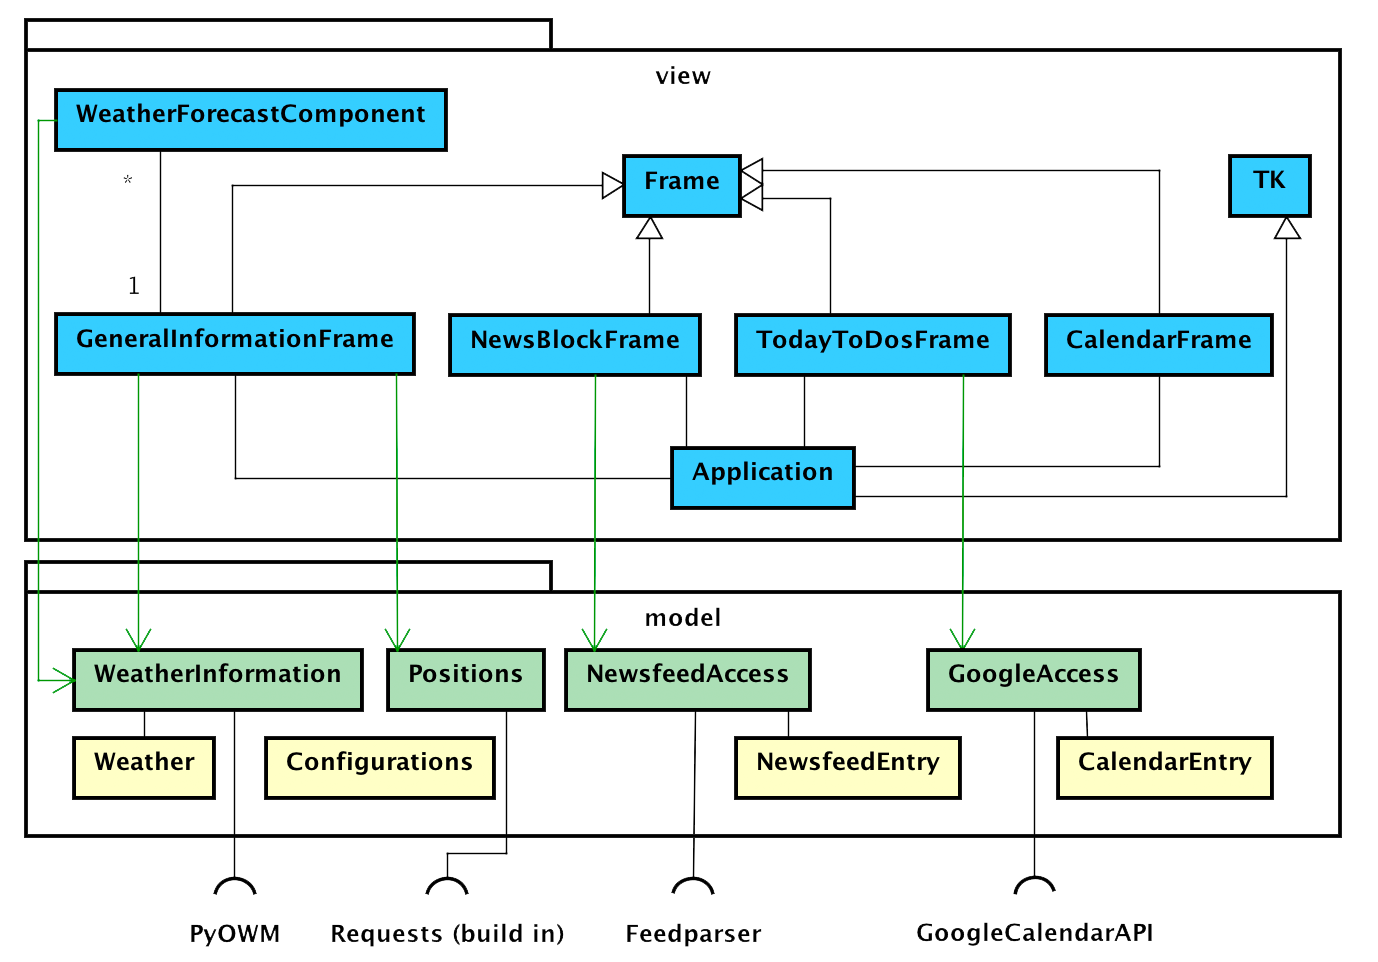
\includegraphics[width=0.7\linewidth]{bilder/umlDiagramNoBackground}
	\caption[UML-Diagramm: Klassenaufbau der Hauptapplikation]{UML-Diagramm: Klassenaufbau der Hauptapplikation}
	\label{fig:umldiagramClasses}
\end{figure}

\textcolor{green}{\textbf{Struktur passt nicht so ganz!!! - CalendarFrame rausschmeißen}}   

Die View-Schicht implementiert als wesentliches Element die Klasse \textit{Application}, die von \textit{Tk} erbt. 
\textit{Application} enthält, wie zuvor erwähnt die Frames \textit{NewsBlockFrame}, \textit{TodayToDosFrame}, sowie das \textit{GeneralInformationFrame}. Das \textit{GeneralInformationFrame} nutzt für die Darstellung die \textit{WeatherForeCastComponent}, während die aktuelle Urzeit und das Datum direkt über das Betriebssystem ermittelt und ausgegeben werden. Dies geschieht durch das Kommando \textit{time.strftime(\grq \%H:\%M\grq)} in Zeile 12 (vgl. \autoref{lst:structGeneralFrame}). Hierbei liefert die Methode die aktuelle Uhrzeit in dem Format Stunde:Minute zurück. In der darauf folgenden Zeile wird überprüft, ob sich die aktuell angezeigte Uhrzeit mit der neu Bestimmten übereinstimmt. Ist dies nicht der Fall, so wird in Zeile 14 über das Attribut \textit{$text=new\_ time$} die Aktualisierung vorgenommen.
Zeile 16 sorgt für den erneuten Methodenaufruf nach 200 Millisekunden.

\begin{minipage}{\textwidth}
	\lstinputlisting[frame=single, language=python, style=myPython, escapeinside={(*}{*)}, caption={GeneralInformation Frame},label=lst:structGeneralFrame]{codesnippets/frameExample.py}
\end{minipage}
 
 Die Model-Schicht importiert und hält die anzuzeigenden Daten vor, ebenso wie zentrale Informationen zur Darstellung, die als globale Variablen in \textit{Configurations} vorgehalten werden. \textit{Positions} ist eine Klasse, die über die IP-Adresse des WLAN-Interfaces die Position ermittelt, um daraus implizit den aktuellen Ort für die Wettervorhersage zu ermitteln. Diese Information benötigt die Klasse \textit{WeatherInformation}, um über die \textbf{Py}thon \textbf{O}pen \textbf{W}eather \textbf{M}ap (PyOWM) (vgl. Quelle) die aktuelle Wettervorhersage für den ermittelten Ort anzufragen. PyOWM selbst ist ein Python Wrapper zur Nutzung der Open Weather Map. Die erforderliche Kommunikation zur Ermittlung der Daten ist in (vgl. \autoref{fig:umldiagramClasses}) dargestellt.
 Die Klasse \textit{GeneralInformationFrame} fordert über die Methode \textit{getWeather} die Wetterdaten von der Klasse \textit{WeatherInformation} an. Diese startet über PyOWM eine Web-Anfrage bei der Open Weather Map. Nach Empfang der Daten legt \textit{WeatherInformation} die Informationen als \textit{Weather}-Daten im Model ab und stellt sie so dem \textit{GeneralInformationFrame} zu Verfügung. 


\begin{figure}
	\centering
	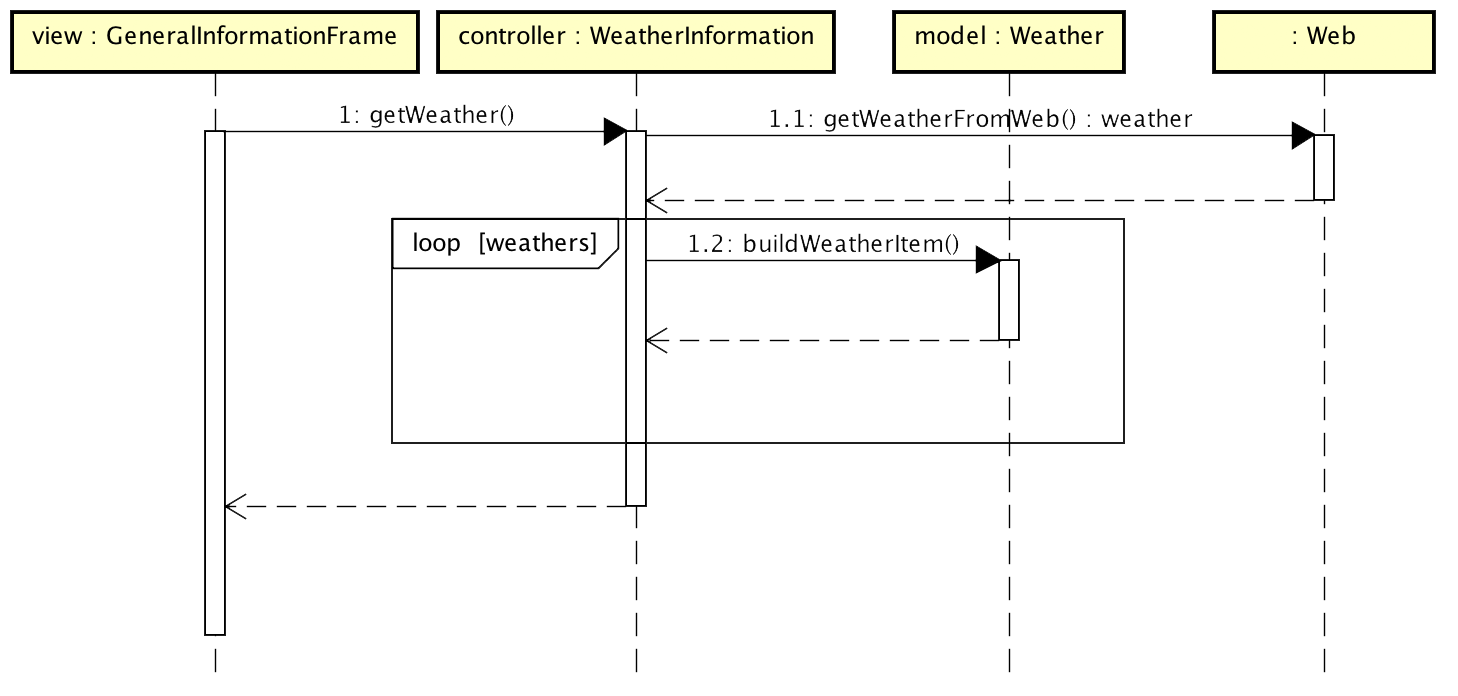
\includegraphics[width=0.7\linewidth]{bilder/sequenceDiagramGettingDataNoBackground}
	\caption{Sequenzdiagramm: Bezug von Daten aus dem Internet}
	\label{fig:sequenzDiagramData}
\end{figure}

\textcolor{green}{\textbf{Abbildung anpassen - MVC raus + Web durch Open Weather Map ersetzen}}   

Analog dazu stellt die Klasse \textit{NewsfeedAccess} Daten, die sie über den Feedparser \textcolor{green}{\textbf{konkretisieren!!!}} abfragt in Form von \textit{NewsFeedEntries} für den \textit{NewsBlockFrame} bereit. Ebenso ruft die Klasse \textit{GoogleAccess} die aktuellen Kalendereinträge über die GoogleCalendarAPI \textcolor{green}{\textbf{konkretisieren!!!}} 
ab und stellt sie als \textit{CalenderEntries} bereit.



\subsection{Das StartUp-Skript}

\section{Der SmartMirror im Einsatz}
\subsection{Inbetriebnahme}
\subsection{Showcase}

\section{Fazit und Ausblick}
